\begin{tikzpicture}[scale=0.75]
    \pgfmathsetmacro{\HEIGHT}{1.5}
    \pgfmathsetmacro{\XSTEP}{3.7}
    \pgfmathsetmacro{\YSTEP}{4.3}
    \pgfmathsetmacro{\YLABEL}{-0.4}
    \pgfmathsetmacro{\NUDGE}{0.5}
    % regarding /includegraphics commands, note /graphicspath in main file
    \node (start2) [] at (0,2*\YSTEP) {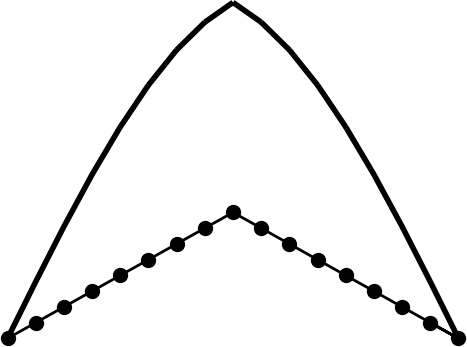
\includegraphics[height=\HEIGHT cm]{start2.png}};
    \node (start2label) [below of = start2, yshift=\YLABEL cm] {$w^2 \ge \underline{\gamma}^2$};
    \node (down2) [] at (1.0*\XSTEP,2*\YSTEP) {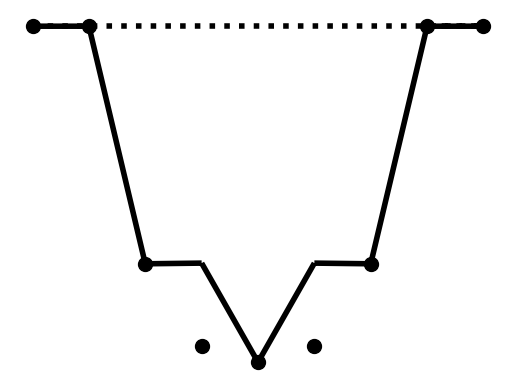
\includegraphics[height=\HEIGHT cm]{down2.png}};
    \node (down2label) [below of = down2, yshift=\YLABEL cm] {$y^2 \ge \underline{\phi}^2$};
    \node (down1) [] at (1.4*\XSTEP,1*\YSTEP) {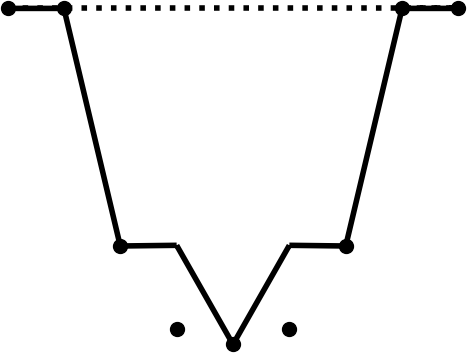
\includegraphics[height=\HEIGHT cm]{down1.png}};
    \node (down1label) [below of = down1, yshift=\YLABEL cm] {$y^1 \ge \underline{\phi}^1$};
    \node (up0) [] at (1.9*\XSTEP,0) {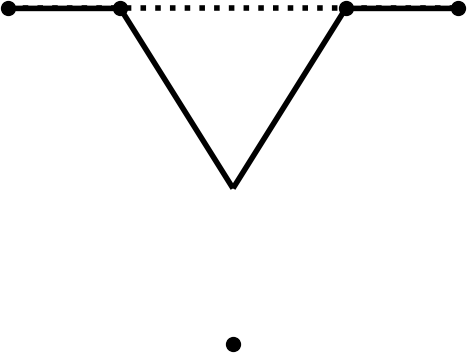
\includegraphics[height=\HEIGHT cm]{up0.png}};
    \node (up0label) [below of = up0, yshift=\YLABEL cm] {$z^0 \ge \underline{\chi}^0$};
    \node (up1) [] at (2.4*\XSTEP,1*\YSTEP) {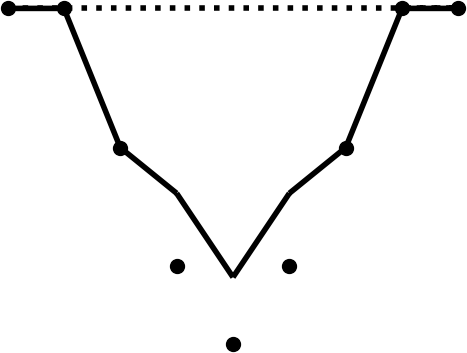
\includegraphics[height=\HEIGHT cm]{up1.png}};
    \node (up1label) [below of = up1, yshift=\YLABEL cm] {$z^1 \ge \underline{\chi}^1$};
    \node (up2) [] at (2.8*\XSTEP,2*\YSTEP) {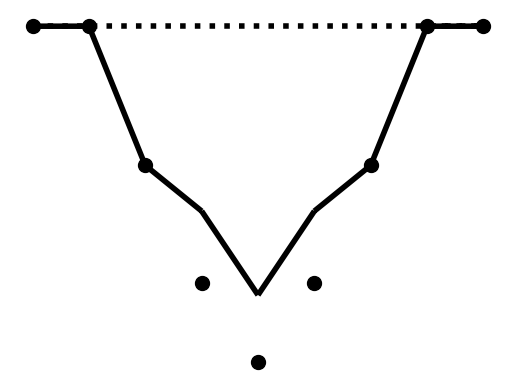
\includegraphics[height=\HEIGHT cm]{up2.png}};
    \node (up2label) [below of = up2, yshift=\YLABEL cm] {$z^2 \ge \underline{\chi}^2$};
    \node (next2) [] at (3.8*\XSTEP,2*\YSTEP) {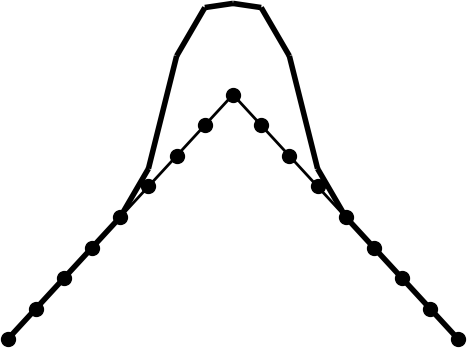
\includegraphics[height=\HEIGHT cm]{next2.png}};
    \node (next2label) [below of = next2, yshift=\YLABEL cm] {$\tilde{w}^2 \ge \underline{\gamma}^2$};
    \graph [edges = {very thick}] {
        (start2) -> (down2)
                 -!- [] (down2label) -> (down1)
                 -!- [] (down1label) -> (up0)
                 -> (up1label) -!- (up1)
                 -> (up2label) -!- (up2)
                 -> (next2)
    };
\end{tikzpicture}
